\subsection{Introduction}\label{subsec:2.3.feat_extr_intro}

Feature Extraction is another element of the MANOLO functionality directed towards the enhancement of AI efficiency. This submodule will provide the user with a set of tools and functions to extract relevant information from the data and represent it in compact features. This results in a memory and computationally efficient representation of the dataset that contains the necessary information to replicate results obtained with the original data. 

Early approaches to feature extraction leverage domain specific hand crafted features like color, texture or shapes for images~\citep{2019_ICSP_featExtrSurv}. These approaches presented poor generalization across datasets and required time-consuming human supervision. Hence, current state-of-the-art has moved towards the exploitation of pre-trained models to extract features from the data~\citep{laion, 2019_CVPR_transferImagenet, 2021_ICML_transferNLP}. Pre-trained models are exposed to a high variety of samples from different domains during training and learn to extract the most relevant features. As a widely adopted practice in the Computer Vision community, practitioners use ImageNet~\citep{imagenet} pre-trained models as an initial data pre-processing step to obtain informative and memory efficient features as representations of the samples. The adaptation of these features to the target domain depends on the similarity between the target and the pre-training, or source, domains~\citep{2018_CVPR_taskonomy}. The direct solution to feature extraction when working with specialized datasets is to train models directly on the target dataset. The main caveat of this approach, apart from increased computational costs, is the reliance on dataset quality; concretely, on annotations quality. An effective approach in this case, is to leverage models that learn the distribution of the data independently from the labels. Variational Auto-Encoders (VAE) are a widely adopted example of these models~\citep{2023_AISTATS_vqvae, 2015_ICLRw_VRAE, 2017_NeurIPS_VQVAE}. Finally, recent advances focus on larger models trained on vasts amounts of data that provide more descriptive and discriminative features at the cost of more computational requirements during training and inference~\citep{2024_Springer_foundation, 2021_ICML_CLIP}.

At the time of this deliverable, this section presents two basic techniques included in the Feature Extraction MANOLO submodule: a pretrained Neural Network (NN), specifically a Convolutional Neural Network (CNN),  and a complex Auto-Encoder (AE) architecture, specifically a Vector Quantized Variational AE (VQ-VAE). These two techniques have the advantage of being easily scalable to different datasets and types of data. The CNN-based feature extractor is a very generic approach that leverages pre-trained weights and is able to accommodate different types of models to address different types of data and modalities. The VQ-VAE-based approach learns the distribution of the data through a training stage that we then use to extract representative features. 

The implementation we are presenting in this version of the deliverable is designed for time-series and image data but simple adaptations in the pre-processing stage allow the models to generalize to other types of data, which will be included in future versions of the deliverable. These two approaches are well suited to exploit synergies with explainability metrics~\cite{2022_ssrn_explain, 2024_Neurocomputing_explain}, which we will also address in the next version of this deliverable. The following subsections will delve into these approaches separately, explaining the associated development methodology, and the results obtained up to this stage.


%%%%%%%%%%%%%%%% Naive/baseline feature extractor %%%%%%%%%%%%%%%%
\subsection{Pre-trained Neural Network as a Feature Extractor}
\label{subsec:2.3_featext_tech1}
The initial iteration of the Feature Extraction MANOLO submodule leverages pre-trained NNs to extract features from data, their discriminative capabilities and adaptability across data types and modalities make these models perfect candidates for this task. There are numerous models trained in diverse and large datasets that can be easily downloaded and used in particular tasks. The models included in this version of the report are Convolutional Neural Networks (CNNs) pre-trained in Computer Vision classification tasks with the ImageNet dataset. However, the range of datasets used for pre-training CNNs is wide, spanning from classification to semantic segmentation. It is worth noting that these features, as it happens with raw data, can be used to train models intended to perform tasks unrelated to that used to train the feature extractor.

The feature extraction procedure presented in this version of the deliverable intends to obtain a reduced representation of a sample as the byproduct of being processed by a CNN. In this manner, we use CNNs as functions that map samples into lower dimensional vectors. The performance achieved when replacing the original dataset with the extracted features heavily depends on the relationship between the target task and the task used to pre-train the feature extractor~\cite{2018_CVPR_taskonomy}. Nonetheless, these extracted features provide a valuable resource-efficient alternative to the full dataset and a competitive starting point for a wide variety of applications and tasks.   


\subsubsection{Methodology}\label{subsubsec:NNfeatExtr_Meth}
We establish a baseline approach to feature extraction by the use of CNNs trained on the 1,000 classes ImageNet classification task, predicting a class probability distribution after the last layer, linear, has its logits activated through a softmax function. In particular and for this report, we focus on two types of architectures: VGG~\cite{2016_ICLR_VGG} and ResNet~\cite{2016_CVPR_ResNet}. To obtain more generic features we discard the last linear layer and its activation function and directly use the output of the previous residual block for ResNet architectures, or linear layer for VGG architectures. 

\subsubsection*{Feature evaluation}
\begin{quote}
In order to evaluate the quality of the features extracted, we have followed a method widely adopted in self-supervised tasks, consisting in training two classifier networks, a linear classifier~\cite{2020_ICML_simple} and a KNN classifier~\cite{2018_CVPR_unsupervised}, with the extracted features. The linear classifier proves the features' ability to linearly separate classes, and the KNN the quality of the feature space in terms of associating sample similarity to semantic class.

Furthermore, as we aim to create compact versions of the dataset by extracting the features from the data, we have also included a non-linear evaluation test for feature fitness for complex classifiers, in terms of model generalization and adaptability. The architecture of the third evaluator is that of  a non-linear classifier composed by two linear layers with a ReLu activation, creating non-linearity between them. Additionally, we include a qualitative evaluation showing the ability of the feature extractors to allocate similar samples close in the feature space. This is a retrieval-based evaluation that, as illustrated later in Section~\ref{subsubsec:NNfeatExtr_Res} in Figure~\ref{fig:exp_feat_extr_retrieval}, shows the closest samples to a few randomly selected query samples. This evaluation is done by measuring distance between samples with the cosine similarity metric.
\end{quote}

\subsubsection*{Experimental setup} 
\begin{quote}
The experiments in this subsection are carried out on the CIFAR-10 dataset for image classification. This dataset consist of 60,000 natural images of 32$\times$32 RGB pixels distributed across ten classes and split into a set of 50,000 samples for training and a set of 10,000 samples for testing. Each of the experiments is done for three different NN architectures: VGG~\cite{2016_ICLR_VGG}, VGG with batch normalization, and ResNet~\cite{2016_CVPR_ResNet}. In each case, we evaluate two different model sizes: for the VGG architecture we chose VGG-11 and VGG-19, and for the ResNet architecture we chose ResNet-18 and ResNet-50. Table~\ref{tab:NN_specs} summarizes the difference in number of parameters between these models. Additionally, given that the selected models are initially trainedo on 256$\times$256 resolution images, we evaluate the performance of featres extracted from an upsampled version of CIFAR-10 images.  
\end{quote}

\begin{table*}[h]
    \centering      
    % \label{tab:NN_specs}
    % \vspace{-8pt}
    % \resizebox{0.95\textwidth}{!}{%
    \caption{\label{tab:NN_specs} Model specifications: number of parameters in millions and feature size.} 
    \begin{tabular}{lccc}
        \hline 
        {Architecture} & {Number of parameters (M)} & {Feature size} \tabularnewline
         \hline
        VGG-11 & 128.77 &  4,096 \tabularnewline
        VGG-11 + BN & 128.77 &  4,096 \tabularnewline
        VGG-19 & 139.57 &  4,096  \tabularnewline
        VGG-19 + BN & 139.58 &  4,096  \tabularnewline
        ResNet-18 & 11.18 & 512 \tabularnewline
        ResNet-50 & 22.51 &  2,048 \tabularnewline
        \hline
    \end{tabular} 
    % \caption{\label{tab:NN_specs} Model specifications: number of parameters in millions and feature size.} 
     % }
\end{table*}

\subsubsection{Results}\label{subsubsec:NNfeatExtr_Res}

The results reported in this section evaluate the fitness of certain CNNs to be part of the MANOLO Feature Extraction submodule. Concretely, the experiments carried out provide a comparison of the feature quality when using different pre-trained and randomly initialized models as feature extractors. The results reported in Table~\ref{tab:feat_extr_results_pretrained} show the reliability of this approach across architectures and the consistency of the results when changing the number of parameters of a model. In particular, Table~\ref{tab:feat_extr_results_pretrained} provides a baseline accuracy of the models directly trained on the CIFAR-10 dataset, and three different accuracy evaluations of the performance of features extracted from the original 32$\times$32 images and of the 256$\times$256 upsampled images. Additionally, Figure~\ref{fig:exp_feat_extr_retrieval} provide a qualitative evaluation that demonstrates the ability of the extracted features to preserve visual similarity between samples. The figure illustrates this by depicting a query image in the first row and its ten closest samples according to the cosine similarity of the extracted features. Note that the top right pane in Figure~\ref{fig:exp_feat_extr_retrieval} shows the closest images when the features are extracted with randomly initialized weights and the top left pane when the features are extracted with a pre-trained model.


\begin{table*}[h]
    \centering       
    % \vspace{-8pt}
    % \resizebox{1.0\textwidth}{!}{%
    \caption[Accuracy metrics for original and upsampled CIFAR-10 images]{\label{tab:feat_extr_results_pretrained} Accuracy metrics (\%) of features extracted with pre-trained weights evaluated in the CIFAR-10 test set for the original image size and for upsampled images.}     
    \begin{tabular}{lccccccc}
        \hline 
        {} & \multicolumn{1}{c}{} & \multicolumn{3}{c}{32$\times$32 images}& \multicolumn{3}{c}{256$\times$256 images}\tabularnewline
        \hline
        % {} & {} & \multicolumn{3}{c}{32 images}& \multicolumn{3}{c}{256 images}\tabularnewline
        % \hline        
        % {Architecture} & {Baseline acc.} & {KNN acc.} & {Linear acc.} & {Non-linear acc.} & {KNN acc.} & {Linear acc.} & {Non-linear acc.} \tabularnewline
        {Architecture} & \multicolumn{1}{c|}{Baseline} & {KNN} & {Linear} & {Non-linear} & \multicolumn{1}{|c}{KNN} & {Linear} & {Non-linear} \tabularnewline
         \hline
        VGG-11 & 91.90  & 60.12 & 61.61 & 66.02  &  75.79 & 85.16  & 84.86 \tabularnewline % https://www.kaggle.com/code/salmaelsayed1/cifar10-vgg11-91-90
        VGG-11 BN & 91.61 & 61.56 & 66.12  & 68.96 & 75.89  &  85.87 &  86.60 \tabularnewline % baseline vgg11 NB rfom https://arxiv.org/pdf/1901.06656v2
        VGG-19 & 94.50 & 58.16 & 61.96 & 64.69  & 77.15  & 84.88  & 84.99 \tabularnewline % baseline vgg19 from https://arxiv.org/pdf/2102.08098v3
        VGG-19 BN & 94.40 & 60.56 & 64.37 & 67.43  & 80.31 & 86.97 & 87.32 \tabularnewline
        ResNet-18 & 94.94 & 56.97 & 66.90 & 69.88  & 80.97  &  86.36 & 87.87 \tabularnewline% baseline ResNet18 from https://arxiv.org/pdf/2011.10951v2
        ResNet-50 & 95.41 & 59.98 & 70.51  & 71.44 & 83.03  &  89.48 &  90.44\tabularnewline
        \hline
    \end{tabular} 
    % \caption{\label{tab:feat_extr_results_pretrained} Accuracy metrics (\%) of features extracted with pre-trained weights evaluated in the CIFAR-10 test set for the original image size and for upsampled images.}      
     % }
\end{table*}

The first evaluation of the extracted features, by means of the performance of a linear classifier trained on the features extracted from the different pre-trained models, presented in Table~\ref{tab:feat_extr_results_pretrained}, range from 61.96\% accuracy to 70.51\% in VGG-19 and ResNet-50 when 32$\times$32 images are used and from 84.88\% to 89.48\% for 256$\times$256 images. Similar results are obtained from the KNN and nn-linear evaluation. This is far from the state-of-the-art results reported for CIFAR-10 when training the same models from scratch, especially when using 32$\times$32 resolution images. The results of the models trained from scratch in CIFAR-10 are reported under Baseline in Table~\ref{tab:feat_extr_results_pretrained} and typically surpass 90\% of accuracy. The computational cost, however, is drastically lower when using pre-trained weights. It is worth noting that re-scaling CIFAR-10 images to 256$\times$256 pixels provides better results at the cost of higher computational demands: a ResNet-18 on a MacBook Pro with an Apple M3 Max chip and a batch size of 256  takes 95.45 seconds to extract the features of 256$\times$256 rescaled CIFAR-10 images and achieves 87.18\% of accuracy in the linear evaluation, while the same model on the original 32$\times$32 images takes 5.72 seconds and achieves 66.9\%. The bottom pane in Figure~\ref{fig:exp_feat_extr_retrieval} provides the qualitative evaluation of the features from the rescaled image. Note that the size of one of the color resized images used is 256$\times$256$\times$3 resulting in roughly 196,000 values while the largest of the features used in this version of the deliverable is 4,096.

Finally, we compare the results from pre-trained models with the results of randomly initialized models in Table~\ref{tab:feat_extr_results_randInit}. The results obtained from randomly initialized models, are considerably lower; while these are still higher than random chance (10\% accuracy), the difference clearly motivates the adoption of pre-trained models and further research in the adaptation of feature extraction approaches across domain and tasks.

\begin{table*}[h!]
    \centering    
    % \label{tab:feat_extr_results_randInit}    % \vspace{-8pt}
    % \resizebox{0.95\textwidth}{!}{%
    \caption{\label{tab:feat_extr_results_randInit} Accuracy of features extracted with randomly initialized weights in the CIFAR-10 dataset.}      
    \begin{tabular}{lccc}
        \hline 
        {Architecture} & {KNN acc. (\%)} & {Linear acc. (\%)} & {Non-linear acc. (\%)}\tabularnewline
         \hline
        VGG-11 & 41.10 &   39.48 &   45.24 \tabularnewline
        VGG-11 BN & 41.08 &   39.48  &  45.27 \tabularnewline
        VGG-19 & 37.79 &   27.39 &   33.07 \tabularnewline
        VGG-19 BN & 37.78 &   27.39 &   33.05 \tabularnewline
        ResNet-18 & 34.98 &  41.16 &  43.70 \tabularnewline
        ResNet-50 & 33.89 &  35.96  &   10.00 \tabularnewline
        \hline
    \end{tabular} 
    % \caption{\label{tab:feat_extr_results_randInit} Accuracy of features extracted with randomly initialized weights in the CIFAR-10 dataset.}       
     % }
\end{table*}

\begin{figure}[h!]
    \centering
    \caption[Qualitative evaluation of features]{\label{fig:exp_feat_extr_retrieval} Qualitative evaluation of features: The top row of each set of samples correspond to a query image and the ten rows beneath to the ten closest samples. The features were extracted with a ResNet-18 with pre-trained weights (top left images), randomly initialized weights (top right images), and pre-trained weights on rescaled images (bottom images). }    
    \begin{tabular}{ll}
        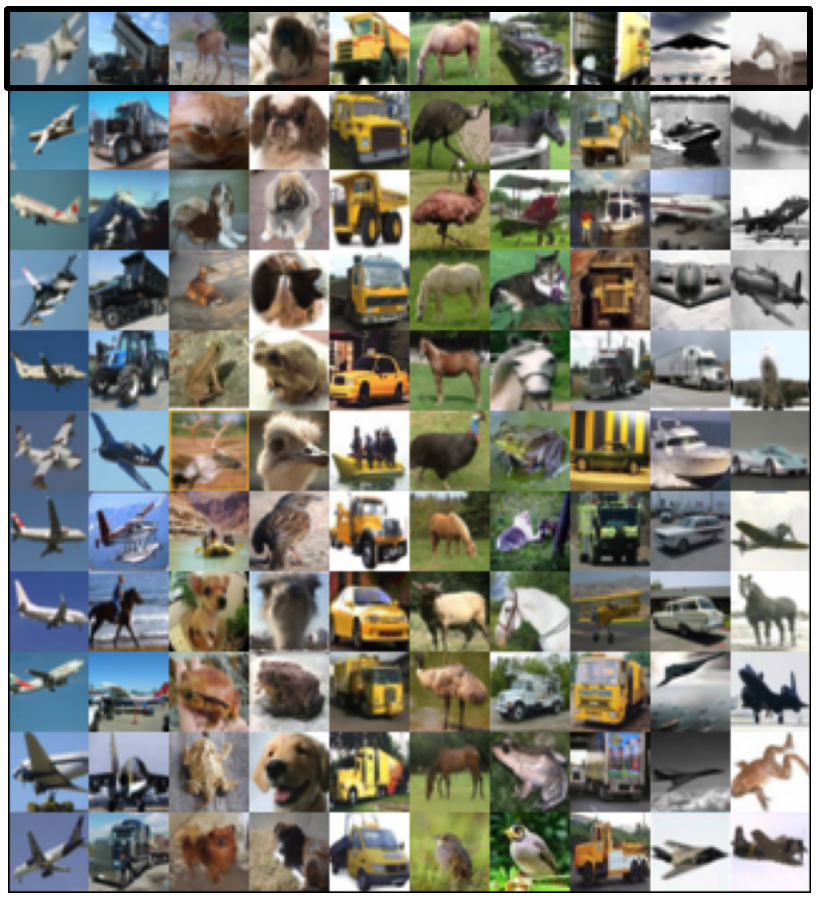
\includegraphics[width=.4\columnwidth]{fig_featureextract/ResNet18_pretrain_32x32.png} & 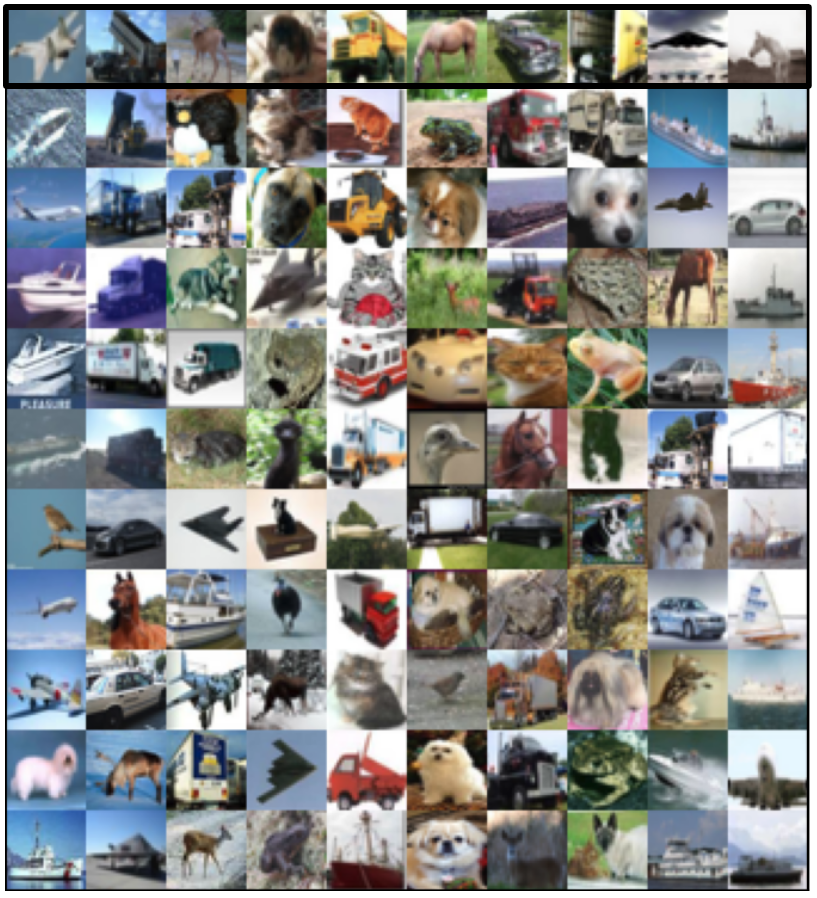
\includegraphics[width=.4\columnwidth]{fig_featureextract/ResNet18_randinit_32x32.png} \\
        \multicolumn{2}{c}{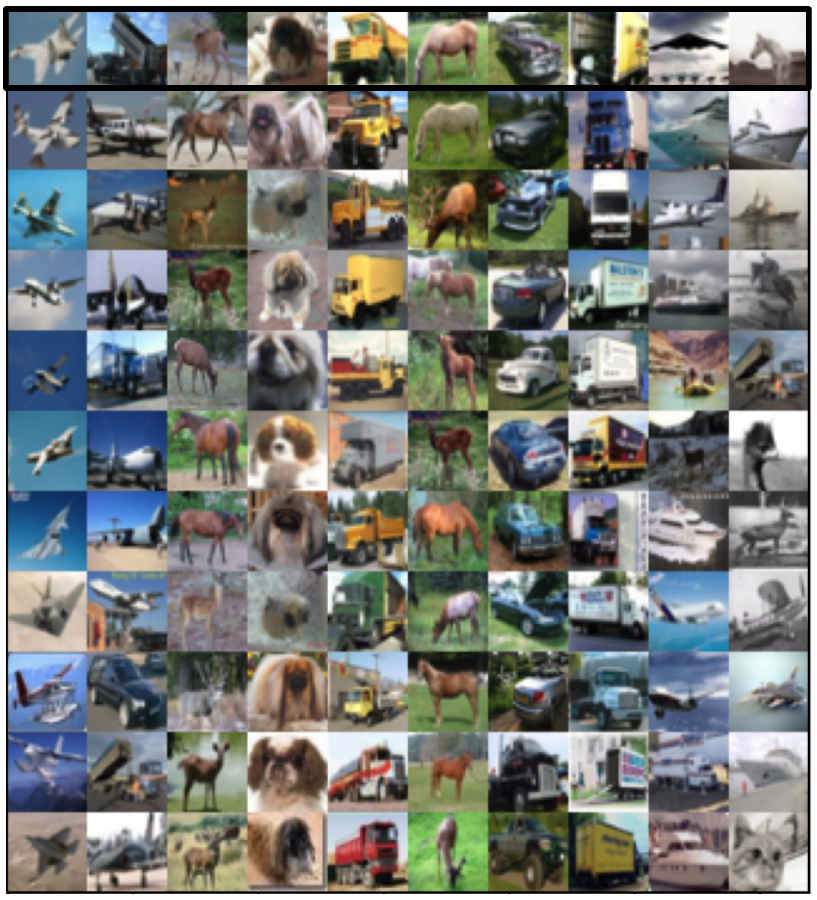
\includegraphics[width=.4\columnwidth]{fig_featureextract/ResNet18_pretrain_256x256.png}} \\
    \end{tabular}
    % \caption{\label{fig:exp_feat_extr_retrieval} The top row of each set of samples correspond to a query image and the ten rows beneath to the ten closest samples. The features were extracted with a ResNet-18 with pre-trained weights (top left images), randomly initialized weights (top right images), and pre-trained weights on rescaled images (bottom images). }
\end{figure}

        
%%%%%%%%%%%%%%%% TimeVQVAE %%%%%%%%%%%%%%%%
\subsection{TimeVQVAE for feature extraction of time-series data.}
\label{subsec:2.3_featext_tech2}

This section describes the approach used to expand the feature extraction capabilities of MANOLO to the time-series domain: variational auto-encoders (VAEs). These are a valuable alternative to extract features in applications where labeled data are scarce, pre-trained models are not available, or the target task is very specific and knowledge transfer is not effective. Concretely, we use TimeVQVAE, the vector-quantized variational auto encoder (VQ-VAE) proposed by Lee et al.~\cite{2023_AISTATS_vqvae}. 

Subsection~\ref{subsubsec:VQVAE_Meth} briefly introduces the VQ-VAE model as a VAE, explaining its value as a feature extractor to be included in the MANOLO Data module, and provides details on the experimental setup used and the evaluation process followed to obtain the results reported in Subsection~\ref{subsubsec:VQVAE_Res}. 
    
\subsubsection{Methodology}\label{subsubsec:VQVAE_Meth}
VQ-VAEs were originally designed for image generation as an improvement of VAE that simplified training and improved the quality of the generated samples~\cite{2017_NeurIPS_VQVAE}. These generative models are trained in an unsupervised manner to reconstruct the input samples, making them independent from possible perturbations in the labeling process. TimeVQVAE as proposed in~\cite{2023_AISTATS_vqvae}, and adopted in this submodule, is an adaptation to time-series data that outperforms contemporary alternatives. Its latent space generates discriminative and representative features that provide a reduced memory-efficient version of the original dataset.
        
VQ-VAEs are a quantized version of traditional VAEs with a discrete latent space that allows for more realistic sample generation. The particular implementation adopted in MANOLO, TimeVQVAE, consists of two training stages. In the first stage an encoder block maps samples to a latent space, a quantizer discretizes the latent space into learned tokens, and a decoder block maps vectors from the latent space back to the sample space. This stage is trained with a reconstruction loss that assures the generation of realistic samples and an MSE minimization loss that optimizes the tokens learned by the quantizer. Then, the second stage uses a bi-directional transformer to learn the prior distribution of the latent space. TimeVQVAE, as VAEs do, produces an output that resembles the input sample while passing through a latent space of reduced dimensionality. This compression of the representations, and quantization in the case of VQ-based models, guides VAEs to learn a mapping function, the encoder, that preserves the most relevant features to reconstruct the input sample.

\subsubsection*{Feature evaluation setup}  
\begin{quote}
To repurpose TimeVQVAE for the MANOLO feature extraction functionality, we leverage the latent space learned by the encoder and use the latent vectors as extracted features. Hence, the trained encoder of the TimeVQVAEs becomes the feature extractor model. Additionally, to homogenize the features and further compress the data, we use a PCA and keep the 50 most relevant components of the extracted features. The evaluation of these features is carried out following the procedure described in Section~\ref{subsubsec:NNfeatExtr_Meth}, i.e. we report accuracy with a linear classifier, with a non-linear classifier, and with a KNN-classifier. In addition, due to the class imbalance in the datasets studied in this section, we report the balanced accuracy metric, as implemented in the scikit-learn library~\cite{scikit-learn}, for these three classifiers~\footnote{\url{https://scikit-learn.org/stable/modules/generated/sklearn.metrics.balanced_accuracy_score.html}}. This metric reports a more accurate measure of the performance of a model when the number of samples in each class is imbalanced.  
\end{quote}

\subsubsection*{Experimental setup}
\begin{quote}
The TimeVQVAE implementation integrated in MANOLO closely follows the architecture and adopts most of the hyperparameters suggested in the original paper~\cite{2023_AISTATS_vqvae}. To increase the data compression capabilities of these technique, we reduced the size of the model by decreasing the size of the hidden dimension and increasing downsampling of the samples. The features extracted are the flattened vectors produced by the encoder. Given the convolutional nature of the encoder, the dimensionality of the resulting features depend on the size of the input samples. To obtain same size features across datasets we post-process the features with a PCA dimensionality reduction and obtain 50 component features, this achieves an additional compression of the data. We use four time-series datasets easily accessible from the tslearn library~\cite{JMLR:v21:20-091}: ECG5000, ElectricDevices, FordA, and FordB. For all the datasets we used the same pre-processing of the data: Min-Max normalized all the samples and rounded all the values to two decimals. We followed the train-validation split defined in the tslearn library and used the train set to train the VRAE and the classifiers for the evaluation, then computed the reported metrics on the validation set.

The ECG5000 dataset~\cite{2000_physiobank_ECG5000} is constituted by 5,000 randomly selected heart bits from a patient with severe congestive heart failure automatically annotated as one of five classes. The distribution of samples is heavily biased towards the first and second class, which have over 4,000 samples between them while the third, fourth, and fifth classes have less than 500 samples altogether. This dataset is often used in medical time-series research for anomaly detection and classification tasks~\cite{2015_ACM_ecg5000InitialPaper, 2022_IEEE_tsmae, 2022_IEEE_lightweight}, where the 5,000 samples are usually split into 4,500 samples for testing and 500 for training. The imbalance of the data labels makes it a challenging dataset well-suited to one of the purposes of MANOLO: address possible biases. Each sample has a length of 140 measurements of a single variable. 

The ElectricDevices dataset, available in the UCR time-series archive~\cite{2019_IEEE_ucr}, is a collection of electricity consumption readings from 251 households sampled in two-minute intervals over a month, resulting in 16,637 samples split into 8,926 samples for the train set and 7,711 for the test set. The samples are annotated into one of seven classes. In this case, five of the classes have around 1,000 samples each while the other two around 2,000 each. This illustrates a less severe type of class imbalance when compared to the ECG5000 dataset. ElectricDevices is a univariate dataset and the length of each sample is 96 measurements. It is commonly used in time-series classification, forecasting, and explainability among others~\cite{2023_Springer_TSandXAI, 2024_IEEE_gmtpm, 2020_IEEE_fastee, 2016_SEKE_time}.

Finally, the FordA and FordB datasets, also from the UCR archive~\cite{2019_IEEE_ucr} are a collection of samples from an automobile subsystem labeled to identify the presence of a particular symptom resulting in a binary classification task. The first dataset is split into a set of 3,601 samples for training and 1,320 for testing, and the second dataset into 3,636 and and 810 for training and testing respectively. All the samples consist of 500 measurements from a single sensor (univariate time series). Additionally, FordB dataset presents a more challenging task than FordA due to the inclusion of noise in the measurements in the test set. These datasets are used in time-series research as benchmarks for binary tasks as well as robustness against noisy measurements~\cite{2021_ICML_voice2series, 2022_arxiv_hypertime, 2023_Springer_deep}.
\end{quote}
            
\subsubsection{Results}\label{subsubsec:VQVAE_Res}
We have evaluated the latent space learned by the TimeVQVAE both qualitatively and quantitatively. The former consist of the standard evaluation used for self-supervised representation learning, described in Section~\ref{subsubsec:NNfeatExtr_Meth}. In this case we use the encoder of the trained TimeVQVAE as a feature extractor and represent each input sample as a vector from the latent space. The latter consist of a PCA and t-SNE visualization of the latent space that illustrates the ability of the encoder to allocate samples from a given class in a particular region of the space, which showcases its potential applications to other tasks such as retrieval or metric-based learning.

Table~\ref{tab:exp_vqvae_1} shows the results of a linear classifier, a KNN classifier and a non-linear classifier trained on the features from the training set extracted with the encoder of the TimeVQVAE, and evaluated on the test set with the available labels. Table~\ref{tab:exp_vqvae_2} reports the performance of the same evaluation procedures under the balanced accuracy metric. This provides an accurate indication of the ability of the TimeVQVAE to extract class-discriminative features. An initial comparison baseline for these results is the performance of random features, for five, seven, and two classes, this would correspond to 20\%, 14\%, and 50\% , reported in Table~\ref{tab:exp_vqvae_2} under Random. Additionally,  under Supervised, Table~\ref{tab:exp_vqvae_2} includes the state-of-the-art results when training a model for classification with the available labels as reported in~\cite{2021_ICML_voice2series, 2023_Springer_TSandXAI}. Finally, the significant decrease in performance when comparing Table~\ref{tab:exp_vqvae_2} and Table~\ref{tab:exp_vqvae_1} illustrates the impact that imbalanced classes have in the training of feature extractors, which will be addressed by approaches introduced in the MANOLO Data Synthesis module described in Section~\ref{subsec:2.3.data_synth_intro} of this report. Note that, given that the class balanced accuracy is not commonly reported in the literature, this table does not include the supervised baseline.


\begin{table*}[h]
    \centering           
    % \label{tab:exp_vqvae_1}    % \vspace{-8pt}
    % \resizebox{0.95\textwidth}{!}{%
    \caption{\label{tab:exp_vqvae_1} Accuracy (\%) of features extracted with the TimeVQVAE encoder.}
    \begin{tabular}{lccccc}
        \hline 
        { } & {Random} & {Supervised} & \multicolumn{3}{c}{TimeVQVAE} \tabularnewline
        \hline 
        {Dataset} & {} & {} & \multicolumn{1}{|c}{KNN} & {Linear} & \multicolumn{1}{c}{Non-linear} \tabularnewline
         \hline
        ECG5000 & {20.00} & {94.62} & 95.00 &  93.90  &  94.40 \tabularnewline
        ElectricDevices & {14.00} & {64.00} & 68.93 &  65.35  & 70.58 \tabularnewline
        FordA & {50.00} & {96.44} & 77.06 & 82.13 & 86.29 \tabularnewline
        FordB & {50.00} & {92.86} & 59.66 & 54.38 & 53.37 \tabularnewline
        \hline
    \end{tabular} 
    % \caption{\label{tab:exp_vqvae_1} Accuracy (\%) of features extracted with the TimeVQVAE encoder.}
     % }
\end{table*}


\begin{table*}[h]
    \centering           
    % \label{tab:exp_vqvae_2}    % \vspace{-8pt}
    % \resizebox{0.95\textwidth}{!}{%
    \caption{ \label{tab:exp_vqvae_2} Class-balanced accuracy (\%) of features extracted with the TimeVQVAE encoder.}
    \begin{tabular}{lcccc}
        \hline 
        { } & {Random} &  \multicolumn{3}{c}{TimeVQVAE}\tabularnewline
        \hline 
        {Dataset} & {} &  \multicolumn{1}{|c}{KNN} & {Linear} & \multicolumn{1}{c}{Non-linear} \tabularnewline
         \hline
        ECG5000 & {20.00} &  54.93 & 46.59 & 47.72 \tabularnewline
        ElectricDevices & {14.00} &  59.50 & 57.35 & 62.88 \tabularnewline
        FordA & {50.00} &  76.70 & 81.81 & 86.10 \tabularnewline
        FordB & {50.00} &  59.55 & 54.01 & 53.26 \tabularnewline
        \hline
    \end{tabular} 
    % \caption{ \label{tab:exp_vqvae_2} Class-balanced accuracy (\%) of features extracted with the TimeVQVAE encoder.}
     % }
\end{table*}

Figure~\ref{fig:exp_vqvae_3} provides the two dimensional t-SNE and PCA visualizations of the extracted features. The image shows that features belonging to the same class align in the feature space. In particular, for ECG500, the visualization show that the two classes with the larger number of samples are separated. The classes with fewer samples also seem to fall in close regions of the space but overlapping the bigger clusters. It is worth noting that this is only a visualization method and not a reliable manner to evaluate the performance of a classifier. The techniques used (PCA and t-SNE) project the features in two-dimensional plots and this remove nuances and details present in the original features in higher dimensional spaces.

\begin{figure}[h]
    % \vskip -0.2in 
    \centering
    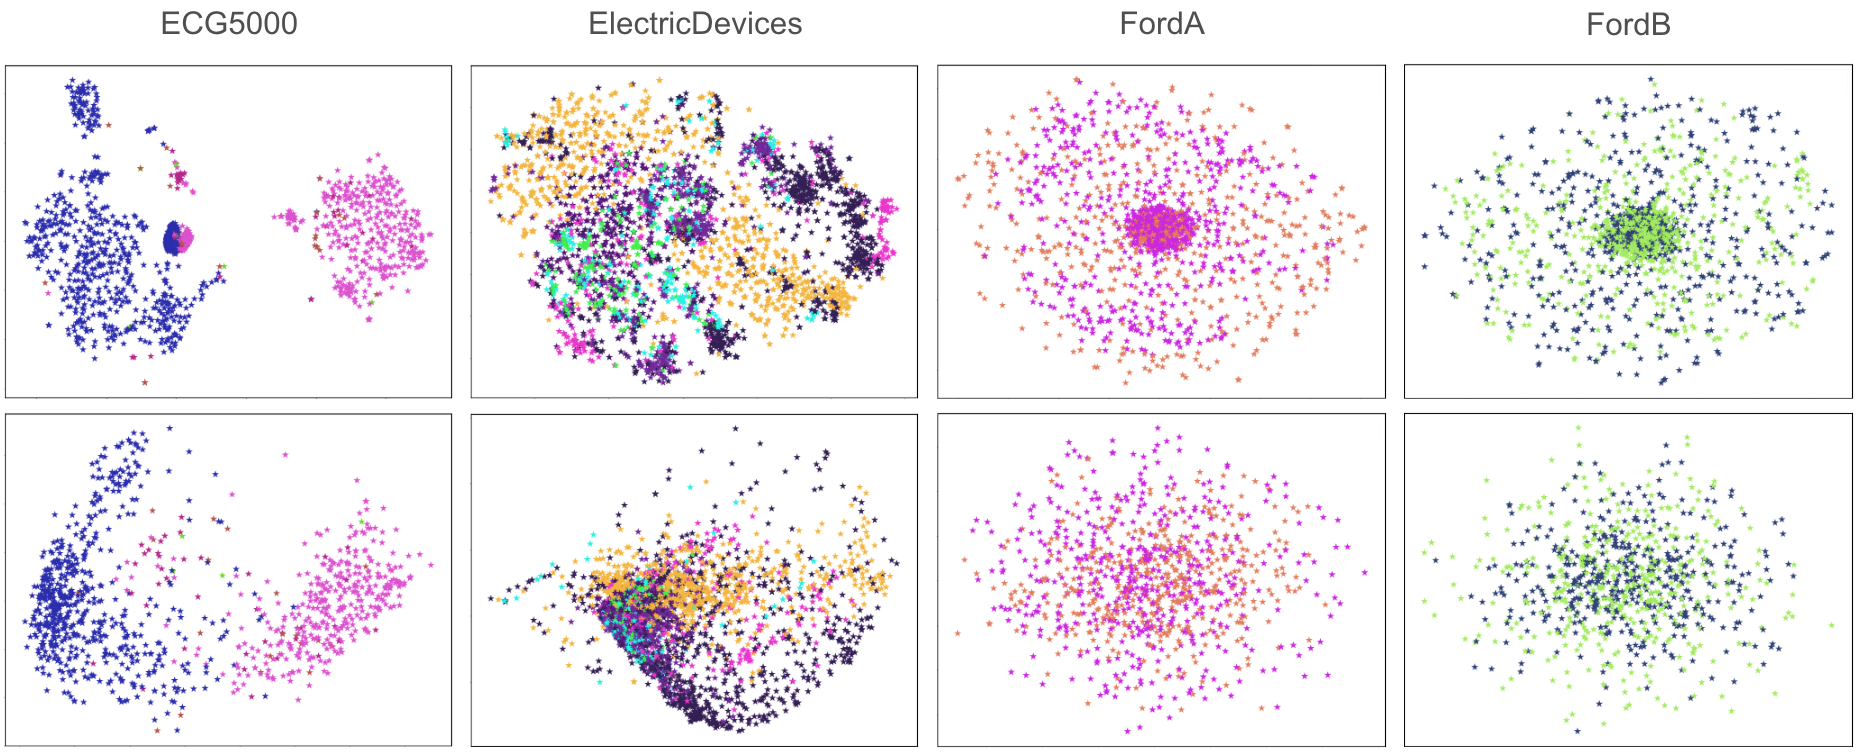
\includegraphics[width=0.95\columnwidth]{fig_featureextract/timeVQAE-tse-pca.png}  
    \caption[T-SNE and PCA visualization of TimeVQVAE features]{\label{fig:exp_vqvae_3} T-SNE (top) and PCA (bottom) visualization of the features extracted with the TimeVQVAE encoder from the four datasets used in this report.}
    % \vspace{-2pt}
    % \caption{\label{fig:exp_vqvae_3} T-SNE (top) and PCA (bottom) visualization of the features extracted with the TimeVQVAE encoder from the four datasets used in this report.}
    % \vskip -0.0in 
\end{figure}
   
%%%%%%%%%%%%%%%% %%%%%%%%%%%%%%%% %%%%%%%%%%%%%%%%
%%%%%%%%%%%%%%%%   Conclusion   %%%%%%%%%%%%%%%%
%%%%%%%%%%%%%%%% %%%%%%%%%%%%%%%% %%%%%%%%%%%%%%%%
% \subsection{Conclusion}
% \label{sec:conclusion}
